\documentclass[11pt, a4paper]{article}

% ==========================================
% 1. PAGE LAYOUT & FONTS
% ==========================================
\usepackage[margin=1.25in]{geometry} 
\usepackage[utf8]{inputenc}
\usepackage[T1]{fontenc}
\usepackage{lmodern} 
\usepackage{setspace}
\setstretch{1.05} 
\usepackage{float}

% ==========================================
% 2. MATH PACKAGES & ENVIRONMENTS
% ==========================================
\usepackage{amsmath, amssymb, amsthm, amsfonts}
\usepackage{mathtools} 

% Define the environments
\newtheorem{assumption}{Assumption}
\newtheorem{proposition}{Proposition}
\theoremstyle{remark} 
\newtheorem{remark}{Remark}

% Custom Math Commands (Add your own here)
\newcommand{\eqdef}{\stackrel{\text{def}}{=}} 
\newcommand{\R}{\mathbb{R}}                   
\newcommand{\E}{\mathbb{E}}                   
\newcommand{\prob}{\mathbb{P}}                
\newcommand{\ind}{\mathbb{I}}                 
\newcommand{\bX}{\boldsymbol{X}}   

% ==========================================
% 3. AUTHORS & AFFILIATIONS (authblk package)
% ==========================================
\usepackage{authblk}
\renewcommand\Affilfont{\small\itshape}
\renewcommand*{\thefootnote}{\fnsymbol{footnote}}

% ==========================================
% 4. ALGORITHMS, FIGURES, & TABLES
% ==========================================
\usepackage{graphicx}
\usepackage{subcaption} 
\usepackage{booktabs}   
\usepackage{algorithm}
\usepackage{algpseudocode}

% Customizing the algorithm output keyword
\algnewcommand{\algorithmicoutput}{\textbf{Output:}}
\algnewcommand{\Output}{\item[\algorithmicoutput]}

% ==========================================
% 5. HYPERLINKS
% ==========================================
\usepackage[colorlinks=true, citecolor=blue, linkcolor=blue, urlcolor=blue]{hyperref}

% ==========================================
% DOCUMENT START
% ==========================================
\begin{document}

% --- TITLE & AUTHORS ---
\title{Lego Minifigs Classification Using Transfer Learning
}

\author[1,2]{% [AUTHOR 1 NAME HERE]
\thanks{% [AUTHOR 1 EMAIL], corresponding author
}}

\author[2]{% [AUTHOR 2 NAME HERE]
\thanks{% [AUTHOR 2 EMAIL]
}}

\author[1,3]{% [AUTHOR 3 NAME HERE]
\thanks{% [AUTHOR 3 EMAIL]
}}

\affil[1]{% [AFFILIATION 1 HERE]
}
\affil[2]{% [AFFILIATION 2 HERE]
}
\affil[3]{% [AFFILIATION 3 HERE]
}

\date{May, 2026
}

\maketitle

% Reset footnote counter to numbers for the rest of the document
\renewcommand*{\thefootnote}{\arabic{footnote}}
\setcounter{footnote}{0}

% --- ABSTRACT & KEYWORDS ---
\begin{abstract}
Identifying and categorizing objects with overlapping visual attributes is a complex challenge in computer vision. 
This project tackles the multilabel classification of Lego minifigures, a scenario where a single subject frequently belongs 
to multiple thematic categories simultaneously (e.g., both "Basic" and "LEGOLAND"). To address this, we implement a transfer 
learning pipeline utilizing a pre-trained ResNet18 convolutional neural network modified with a custom 20-node fully connected head. 
To combat the severe long-tail class imbalance inherent in the dataset, we employ a dual-stage gradient correction strategy: 
inverse-frequency oversampling alongside a weighted Binary Cross-Entropy loss function (BCEWithLogitsLoss), further stabilized 
by geometric data augmentations. The model's performance was evaluated using the F1-score, demonstrating high predictive efficacy 
for themes with distinct morphological features (such as Friends or Duplo) while highlighting the mathematical difficulty of 
isolating visually generic themes (such as Castle). Finally, Gradient-weighted Class Activation Mapping (Grad-CAM) was utilized
 to verify model interpretability, confirming that the network successfully learned to base its predictions on logical, structural 
 features rather than relying on background artifacts or data leakage.
\end{abstract}

%\vspace{0.5cm}
%\noindent\textbf{Keywords:} % [KEYWORD 1, KEYWORD 2, KEYWORD 3, ...]

%\vspace{0.5cm}

% --- MAIN TEXT ---
\section{Introduction}

This project constructs an end-to-end deep learning computer vision pipeline for image classification, using
a pre-trained architecture via transfer learning. We build our model on a Lego Minifigure dataset containing 17632
different figures from various set themes.

\begin{figure}[htbp]
    \centering
    % --- LEFT SIDE: JSON (Plain Text) ---
    \begin{subfigure}[b]{0.55\textwidth}
        \centering
        \small 
\begin{verbatim}
{
  "id": 2740,
  "name": "Truck Driver with Brown Beard...",
  "link": "/minifigs/4j001/truck-driver...",
  "year": 2003,
  "img_url": "https://img.bricklink.com/...",
  "category": "For Juniors",
  "themes": [
    "4 Juniors"
  ]
}
\end{verbatim}
        \caption{JSON Metadata}
        \label{fig:json_source}
    \end{subfigure}
    \hfill
    % --- RIGHT SIDE: IMAGE ---
    \begin{subfigure}[b]{0.2\textwidth}
        \centering
        \includegraphics[width=\textwidth]{../data/images/4J001.jpg} 
        \vspace{0cm} % Adds a little vertical breathing room if needed
        \caption{Visual Representation}
        \label{fig:visual_rep}
    \end{subfigure}
    
    % --- MAIN FIGURE CAPTION ---
    \caption{Data pipeline inputs. The raw JSON metadata (a) is paired with its corresponding image (b) to form a single training instance.}
    \label{fig:data_example}
\end{figure}

The original data comes from two different files (see Figure 1). The first one is a JSON file containing all 
information about one lego minifigure, including its name, release year, category, existing themes and values. 
The second file contains the image of that figure, in a JPEG format. As described in a JSON file, a minifigure can have
a varied number of different themes (e.g., Gears, Star Wars). Our task is to predict the set of themes associated with a given figure. To achieve this,
we first encode our raw data using MultilabelBinarizer to turn our initial theme list into a binary vector. 
We assessed at the frequency of theme counts and chose the top 20 themes to ensure that each theme has sufficient representation across all data splits.
Furthermore, we employ further techniques to prevent the negative effects of
 class imbalance, which will be addressed in the coming section.


\begin{figure}[htbp] % h=here, t=top, b=bottom, p=page of its own
    \centering
    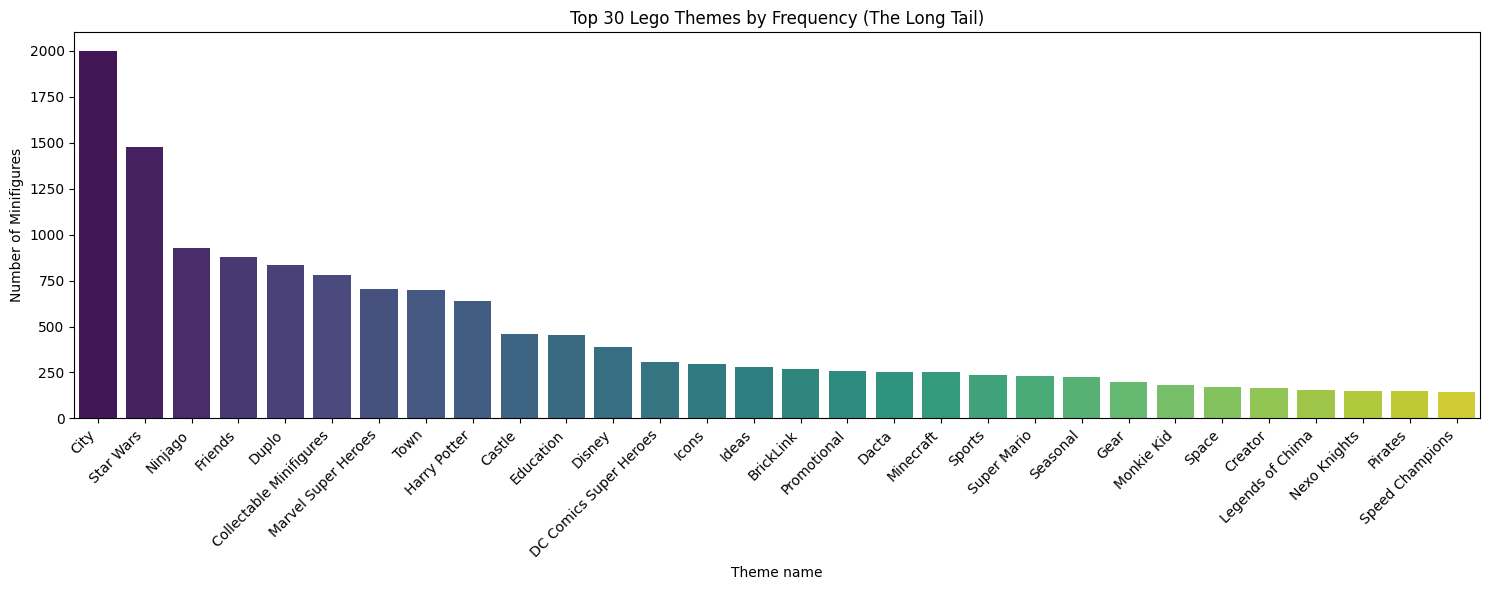
\includegraphics[width=0.8\textwidth]{../outputs/plots/theme_frequency.png} 
    \caption{Frequency of top 30 minifigure themes}
    \label{fig:f1_scores}
\end{figure} 

\section{Methodology}
\subsection{Architecture \& Transfer Learning}
We utilize ResNet-18 \cite{resnet}, pre-trained on the ImageNet dataset \cite{imagenet}, 
as our choice of base model for transfer learning. A defining characteristic of 
the ResNet architecture is its use of residual (skip) connections. These connections 
bypass intermediate layers, effectively mitigating the vanishing gradient problem and 
allowing for the stable training of deep networks. ResNet-18 has a compact design, 
computationally efficient enough for training on consumer-grade hardware. Furthermore, 
it acts as a robust feature extractor due to its early layers being already capable of 
detecting edges, curves, and basic shapes. The convolutional layers are frozen, leaving 
the pre-trained weights untouched. 

\begin{figure}[htbp] % h=here, t=top, b=bottom, p=page of its own
    \centering
    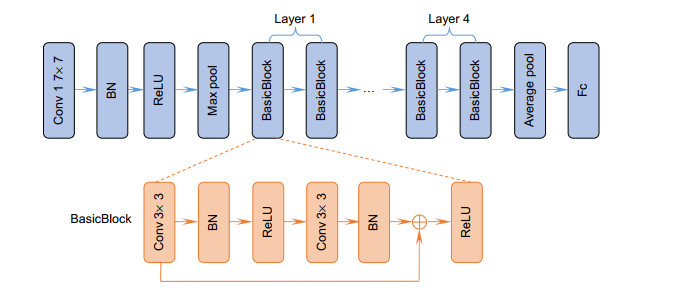
\includegraphics[width=0.8\textwidth]{../outputs/plots/resnet18_architecture.jpg} 
    \caption{ResNet18 architecture}
    \label{fig:f1_scores}
\end{figure} 

We reconstruct this model to fit our project goal by replacing the final fully connected 
layer with a newly initialized, untrained \texttt{nn.Linear} layer, outputting exactly 
20 nodes, one for each predefined theme.

\subsection{Loss Formulation}
For our choice of loss function, we make the assumption that the themes corresponding to 
a certain Lego minifigure are independent of each other. That is, the presence of each 
theme is the outcome of an independent Bernoulli trial. To accommodate this, we use a 
Binary Cross-Entropy loss function combined with Logits (\texttt{BCEWithLogitsLoss}). 

Unlike a Softmax function, which forces the outputs to sum to 1, 
this approach independently applies a Sigmoid activation function, 
$\sigma(\cdot)$, to every output node. For a single image, the multi-label 
loss $\mathcal{L}$ across $C$ total classes (where $C=20$) is defined mathematically as:

\begin{equation}
    \mathcal{L} = -\sum_{c=1}^{C} \left[ y_c \log(\sigma(\hat{y}_c)) + (1 - y_c) \log(1 - \sigma(\hat{y}_c)) \right]
\end{equation}

\noindent where $y_c \in \{0, 1\}$ is the ground-truth binary label for
 class $c$, and $\hat{y}_c$ is the raw logit prediction from the neural
  network. This allows the model to predict high probabilities for multiple 
  themes simultaneously.
\subsection{Handling Class Imbalance}
In a real-world setting, themes follow a long-tail distribution; some themes (like Star Wars or City)
have a significantly larger number of images compared to others. To handle this, we implement a two-pronged mathematical approach
to force the model to respect minority classes.

First, we perform gradient starvation prevention by using WeightedRandomSampler. By using an inverse-frequency sampler with custom weights,
we ensure that rare figures are oversampled and appear consistently in training.

Second, we constructed a custom pos\_weight tensor, which was fed into our loss function. This heavily penalizes the optimizer if it incorrectly 
outputs a probability approaching zero for a rare class, forcing it to aggressively update its weights when it ignores a minority theme.

\subsection{Data Augmentation}
We apply data augmentation by utilizing random horizontal flips and random rotation up to 15 degrees across our data splits to artificially expand the dataset
and prevent the model from memorizing exact pixel layouts.

\section{Experiments and Results}

\subsection{Evaluation Metrics}
During training and validation, we employ our standard loss and accuracy as means of measuring model performance.
However, for testing on our final data split, we choose to utilize F1-score instead, as standard confusion matrices
are invalid for multilabel tasks, and using F1-score would give us a balance between Precision and Recall, which makes it 
the more mathematically rigorous choice.
\subsection{Quantitative Results}
We first discuss our training metrics, which were recorded during our 20-epoch run due to computational constraints.
As can be seen from Figure 4, our training loss appeared to decrease steadily in a curve, before reaching a point where all improvements were marginal.
In contrast, our validation loss appeared to reach a minimum during our 15th epoch before shooting up, indicating possible overfitting 
during our latter runs. Accuracy metrics showed the same trend, with the 15th epoch having the lowest difference between our training and validation accuracy, 
with possible signs of overfitting appearing as our epochs increased. We saved our best-performing model and used said model to evaluate on our test set.
For this particular case, the best-performing model achieved an 80\% accuracy with a loss of 0.038 on our validation set, decreasing by 20\% from our initial validation loss. 

\begin{figure}[htbp] % h=here, t=top, b=bottom, p=page of its own
    \centering
    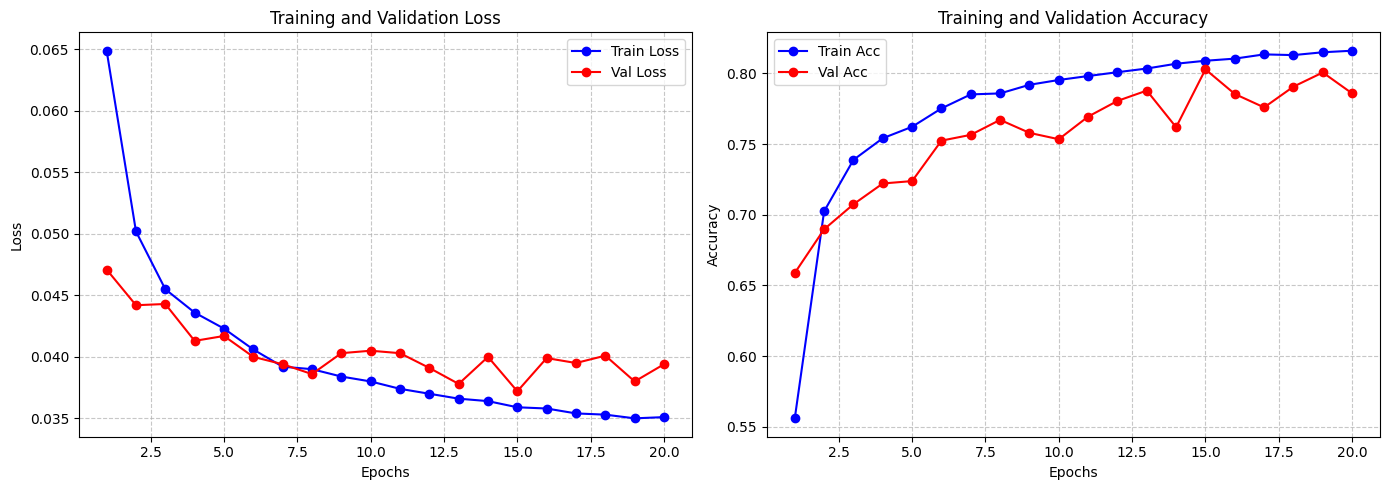
\includegraphics[width=0.8\textwidth]{../outputs/plots/training_validation_loss.png} 
    \caption{Training and validation loss}
    \label{fig:f1_scores}
\end{figure} 

As illustrated in Figure 5, the model achieved varying levels of success across 20 themes. It performed exceptionally well on distinct themes such as 
Friends, Minecraft, Duplo and Star Wars. These are themes with highly unique structure differences, like Minecraft's blocky features
or Friends' unique hairpieces that the model identified efficiently. In contrast, it struggled with Castle, Icons and BrickLink, possibly 
due to sample scarcity and high visual overlap with other generic themes.

\begin{figure}[H] % h=here, t=top, b=bottom, p=page of its own
    \centering
    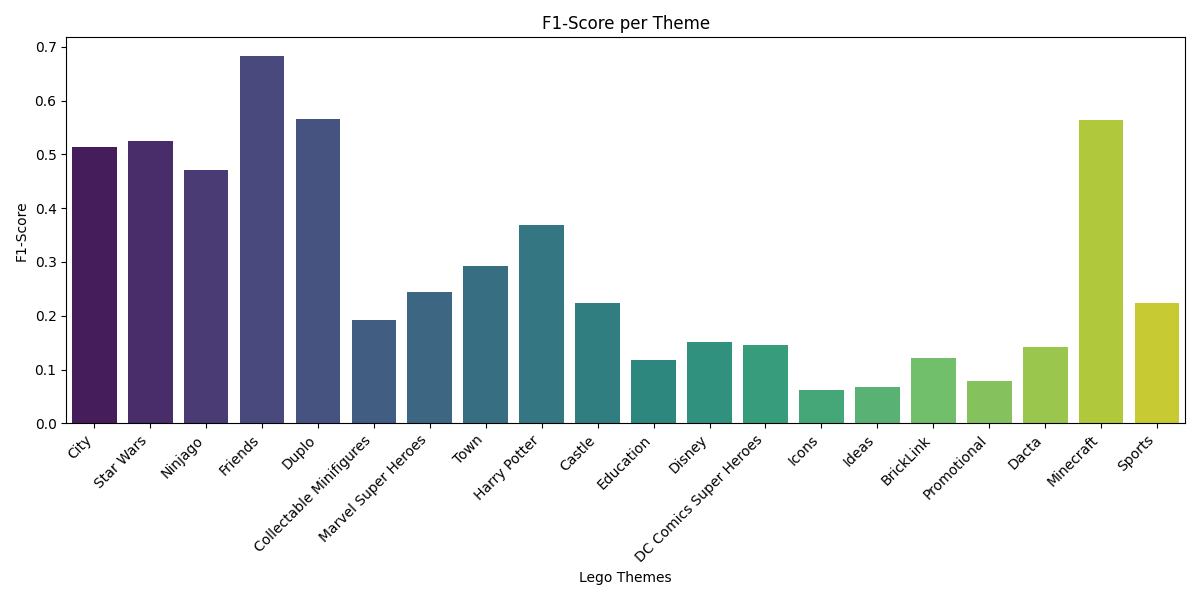
\includegraphics[width=0.8\textwidth]{../outputs/plots/f1_scores_20260408_090920.png} 
    \caption{F1-scores on test set}
    \label{fig:f1_scores}
\end{figure} 

\section{Model Interpretability}
To ensure the model is learning actual Lego features and to get a better understanding of the heuristics employed by our CNN, 
we implemented Gradient-Weighted Class Activation Mapping (Grad-CAM) \cite{gradcam}, which visualizes the spatial gradients of the final convolutional layer 
to show exactly where the model focuses when making a prediction.

\begin{figure}[htbp] % h=here, t=top, b=bottom, p=page of its own
    \centering
    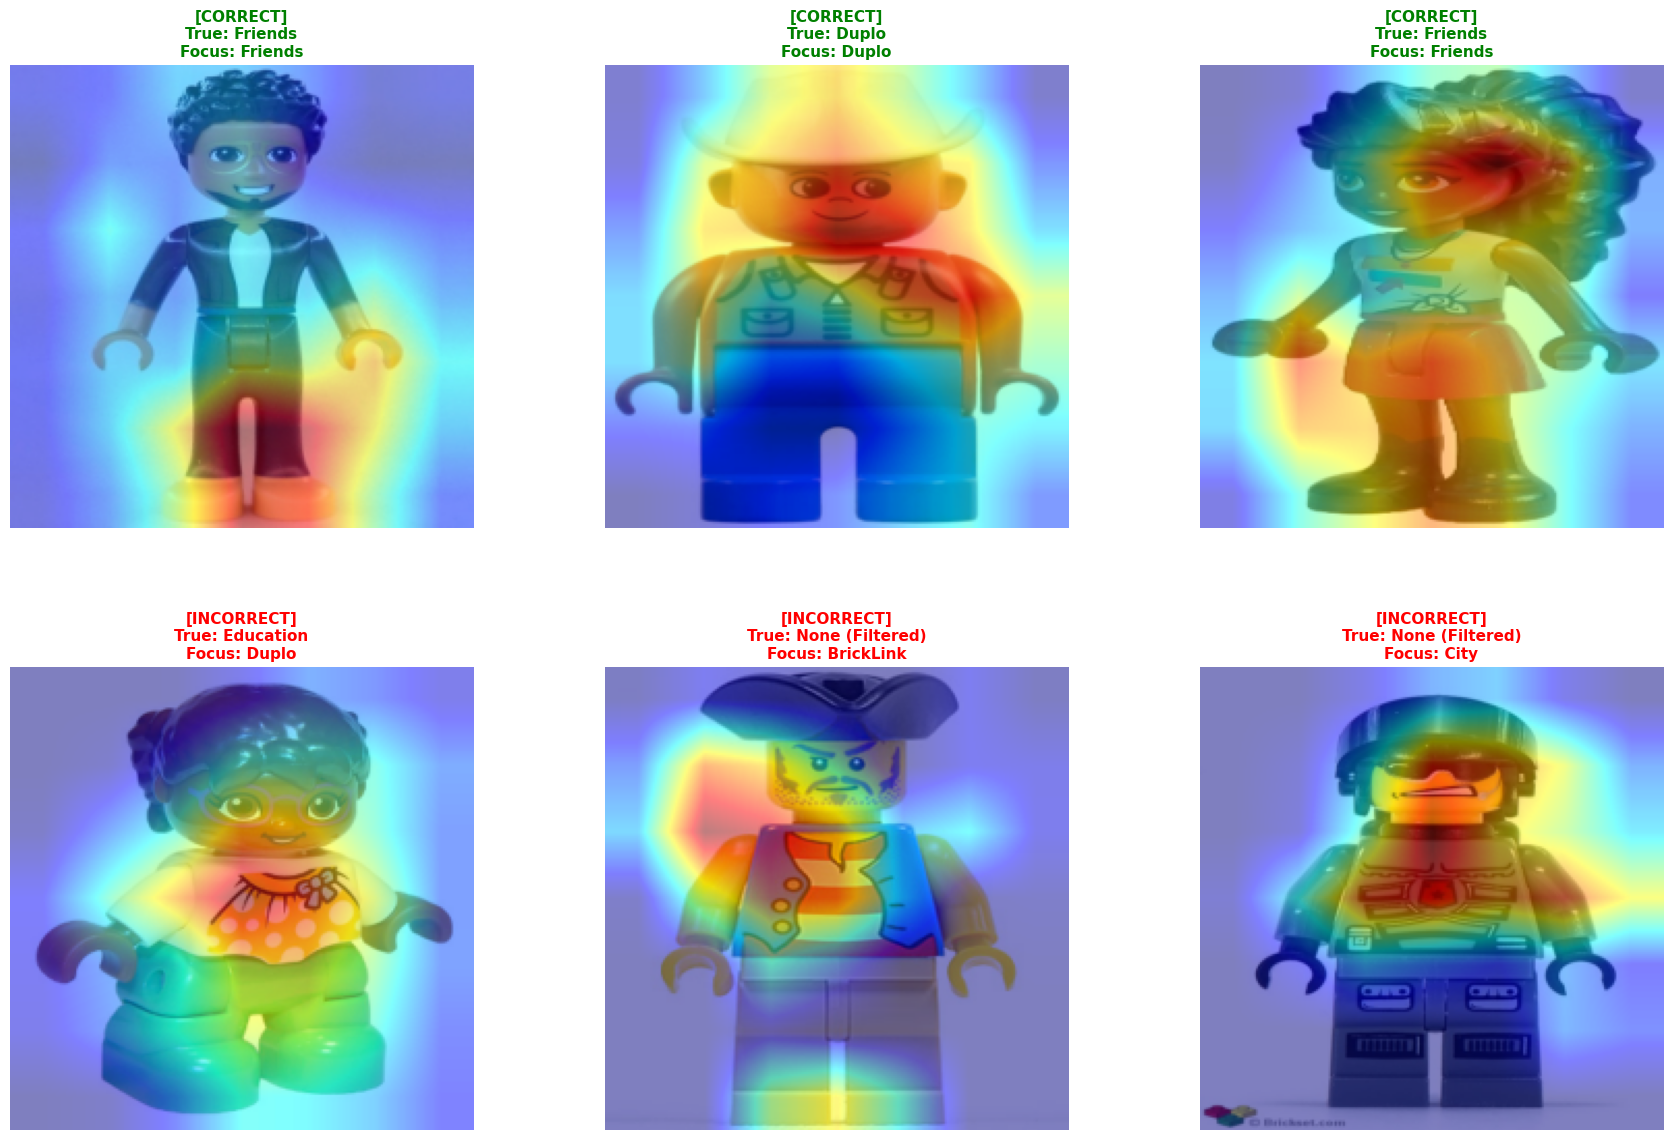
\includegraphics[width=0.8\textwidth]{../outputs/plots/gradcam_comparison_20260408_090920.png} 
    \caption{Grad-CAM interpretability result}
    \label{fig:f1_scores}
\end{figure}

From Figure 6, we can see that, for correct guesses, the model successfully learned discriminative, structural features. For the 
Friends figures, it consistently highlighted unique hairpieces and torso shapes. For the Duplo figures, it recognizes the oversized facial proportions.
The failures are also logical. In cases where the model incorrectly guessed Duplo for an Education figure, the Grad-CAM confirmed the model 
was looking at the oversized head and facial styling features which are visually identical to the Duplo themes. This proves that the model's 
logic is visually sound, even when the ground-truth label differs.

\section{Conclusion}
In conclusion, by employing a transfer-learning architecture and different class-weighting techniques, we have successfully built a model capable of handling a multilabel problem.
 This sets the groundwork
for future possible work, such as exploring more complex model architectures (e.g., Vision Transformers) to improve our performance, 
utilizing different techniques to deal with class imbalance, or diving deeper into different target objectives, like regression on manufacturing year.

% ==========================================
% REFERENCES
% ==========================================
\begin{thebibliography}{9}

\bibitem{resnet}
He, K., Zhang, X., Ren, S., \& Sun, J. (2016). 
\textit{Deep residual learning for image recognition}. 
In Proceedings of the IEEE conference on computer vision and pattern recognition (pp. 770-778).

\bibitem{imagenet}
Deng, J., Dong, W., Socher, R., Li, L. J., Li, K., \& Fei-Fei, L. (2009). 
\textit{ImageNet: A large-scale hierarchical image database}. 
In 2009 IEEE conference on computer vision and pattern recognition (pp. 248-255). IEEE.

\bibitem{gradcam}
Selvaraju, R. R., Cogswell, M., Das, A., Vedantam, R., Parikh, D., \& Batra, D. (2017). 
\textit{Grad-CAM: Visual explanations from deep networks via gradient-based localization}. 
In Proceedings of the IEEE international conference on computer vision (pp. 618-626).

\bibitem{pytorch}
Paszke, A., Gross, S., Massa, F., Lerer, A., Bradbury, J., Chanan, G., ... \& Chintala, S. (2019). 
\textit{PyTorch: An imperative style, high-performance deep learning library}. 
Advances in neural information processing systems, 32.

\bibitem{scikit-learn}
Pedregosa, F., Varoquaux, G., Gramfort, A., Michel, V., Thirion, B., Grisel, O., ... \& Duchesnay, E. (2011). 
\textit{Scikit-learn: Machine learning in Python}. 
Journal of machine learning research, 12(Oct), 2825-2830.

\bibitem{brickset}
Brickset. (2024). \textit{Brickset: The LEGO Minifigure Database}. 
Retrieved from \url{https://brickset.com/}

\end{thebibliography}

% --- EXAMPLE EQUATION ---
%\begin{equation}
    % [EQUATION MATH HERE]
%\end{equation}

% --- EXAMPLE ASSUMPTION ---
%\begin{assumption}[% [ASSUMPTION NAME/LABEL HERE]
%]
% [ASSUMPTION TEXT HERE]
%\end{assumption}

% --- EXAMPLE REMARK ---
%\begin{remark}
% [REMARK TEXT HERE]
%\end{remark}

% --- EXAMPLE TABLE ---
%\begin{table}[h]
%    \centering
%    \begin{tabular}{ll|ccc}
%        \toprule
%        % [TABLE HEADERS HERE] \\
%        \midrule
        % [TABLE ROW 1 HERE] \\
        % [TABLE ROW 2 HERE] \\
%        \bottomrule
%    \end{tabular}
%    \caption{% [TABLE CAPTION HERE]
%    }
%    \label{tab:% [TABLE LABEL HERE]
%    }
%\end{table}

% --- EXAMPLE ALGORITHM ---
%\begin{algorithm}[h]
%\caption{% [ALGORITHM TITLE HERE]
%}
%\begin{algorithmic}[1] 
%\Require % [INPUT CONDITIONS/DATA HERE]
%\For{% [LOOP CONDITION HERE]
%}
%    \State % [STEP DEFINITION HERE]
%    \If{% [IF CONDITION HERE]
%    }
%        \State % [STEP DEFINITION HERE]
%    \EndIf
%\EndFor
%\Output % [OUTPUT DEFINITION HERE]
%\end{algorithmic}
%\end{algorithm}

% --- BIBLIOGRAPHY ---
% \bibliographystyle{plain} % Or your chosen style
% \bibliography{references} % Your .bib file name here

\end{document}